%%%%%%%%%%%%%%%%%%%%%%%%%%%%%%%%%%%%%%%%%%%%%%%%%%%%%%%%%%%%%%%%%%%%%%%%
\chapter{Local Search for Group-Closeness Maximization on Big Graphs}
\label{ch:group-closeness-local-search}
% Labels: heuristic, static, distance-based (closeness), sequential
%%%%%%%%%%%%%%%%%%%%%%%%%%%%%%%%%%%%%%%%%%%%%%%%%%%%%%%%%%%%%%%%%%%%%%%%

%% For the examples with tikz %%
\input{sources/figures/bigdata-graph.tex}

\section{Introduction}
\label{sec:lsh-gc-intro}
Closeness centrality is one of the oldest and most widely-used vertex
centrality measures (see Ref.~\cite{bavelas1948mathematical} and
\Cref{ch:dyn-topk}). It is defined as the
reciprocal of the average shortest-path distance from
a vertex to all the others -- see \Cref{eq:def:closeness}.

Group-closeness can be interpreted as a special case (on graphs)
of the well-known $k$-Median problem for facility location.
Example of applications include: (i) retailers that want to advertise
their products via social media; promoters could be selected as the
group of $k$ members with highest centrality in order to maximize the
influence over the other members~\cite{DBLP:journals/isci/ZhuWWZ14};
(ii) in P2P networks, shared resources could be placed on $k$ peers so
that they are easily accessible by others~\cite{DBLP:journals/pe/GkantsidisMS06};
(iii) in citation networks, group centrality measures can be employed as
alternative indicators for the influence of journals or papers within
their research field~\cite{DBLP:journals/jasis/Leydesdorff07a}.

The problem of finding the group of $k$ vertices with highest group-closeness
(group closeness maximization) is shown to be
\np-hard~\cite{DBLP:conf/adc/ChenWW16}. While exact algorithms to find a group
with maximal closeness are known -- \eg algorithms based on Integer Linear
Programming (ILP)~\cite{DBLP:conf/alenex/BergaminiGM18} -- they do not scale to
graphs with more than a few thousand edges. Hence, in practice, groups with
high closeness centrality are computed through
heuristics~\cite{DBLP:conf/adc/ChenWW16,DBLP:conf/alenex/BergaminiGM18}.

\paragraph{Related Work}
%
For group-betweenness maximization, sampling-based algorithms have been
proposed~\cite{DBLP:conf/kdd/MahmoodyTU16,DBLP:conf/kdd/Yoshida14}. An
extensive analysis of algorithms for group-betweenness estimation is provided
by Chehreghani \etal~\cite{DBLP:conf/bigdataconf/ChehreghaniBA18}, who also
introduce a new algorithm based on an alternative definition of distance
between a vertex and a set of vertices.

Concerning group-closeness maximization, in Ref.~\cite{DBLP:conf/www/ZhaoLTG14}
the definition of group-closeness differs from the original one and only serves
as an estimate of the original -- we use the latter, defined in
\Cref{eq:prelim:gclos}, which is widely accepted. Therefore, their \np-hardness
and submodularity proofs do not necessarily carry over to the original
definition. In fact, the standard group-closeness is not submodular (see
\Cref{lemma:prelim:gclos-not-submod}). Hence, submodular optimization results
in~\cite{DBLP:conf/focs/Vondrak09} do not apply to this case directly.
%
Chen \etal~\cite{DBLP:conf/adc/ChenWW16} argued that group-closeness
maximization is \np-hard by relating it to the \np-hard $k$-means problem.
Their proposed greedy algorithm was later improved by Bergamini
\etal~\cite{DBLP:conf/alenex/BergaminiGM18}, who made algorithm more
memory-efficient and exploited the supermodularity of the reciprocal
of group-closeness for search pruning.
%
Exploiting the supermodularity of the reciprocal also works when the distance
function is replaced by the resistance distance (see
\Cref{sec:prelim-resistance-distance}). This leads to the so-called group
\emph{current-flow} closeness, for which Li
\etal~\cite{DBLP:conf/www/0002PSYZ19} proposed approximation algorithms based
on greedy strategies and random projections.

\paragraph{Motivation}
Still, even for group-closeness with the usual graph distance, the greedy
algorithm can be time-consuming on large instances. Indeed, pruning is most
effective when the group is already large. When performing the first addition,
however, the greedy algorithm has to perform one (pruned) SSSP
\emph{for each vertex in the graph} to compute its marginal contribution, and
this phase scales superlinearly in the size of the graph.
As a result, real-world graphs with hundreds of millions of edges still require
several hours to complete.
%
This motivates us to develop new local search heuristics that quickly find
highly central groups of vertices on large-scale real-world
graphs without sacrificing too much solution quality.

\paragraph{Contribution}
%
In this chapter, we develop new heuristic algorithms for group-closeness
maximization. Specifically, we present two
novel local search heuristics that start from an initial group of vertices $S
\subset V$ and perform exchanges of vertices from $S$ and $V \setminus S$ until
a local optima is reached. The first algorithm, \localswaps, requires little
time per iteration but only exchanges vertices locally. The second algorithm,
\growshrink, performs also non-local vertex exchanges, but iterations are more
computationally expensive.

Experiments on unweighted graphs show that \emph{extended} \growshrink, a
variation of \growshrink, computes groups with closeness scores greater than
$\onedigit{\gsPSevenFiveKQualNum}\%$ of the score of a greedy solution while
being $\onedigit{\gsPSevenFiveKSpeed}\times$ faster (results for $k= 10$).
We see \emph{extended} \growshrink as the best trade-off between
speed and solution quality.
%
When quality is not a primary concern, our other algorithms accelerate the
computation by sacrificing solution quality. For example, for groups with size
10 the non-extended variant of \growshrink yields solutions whose quality is
$\numprint{91.1}\%$ compared to the state of the art while being
$\numprint{700.2}\times$ faster.
The speedup varies between $\onedigit{\gsMaxSpeed}\times$
and $\onedigit{\gsMinSpeed}\times$ for groups with sizes 5 and 100,
respectively.
%
On weighted graphs, our algorithms improve both the quality and
the running time performance of the state of the art: for example, for $k = 10$,
they return solutions of $\onedigit{\wGSQualInc}\%$ higher
quality with a $\onedigit{\wGSSpeed}\times$ speedup. Different trade-offs
between quality and running time are possible, we discuss them in
\Cref{sec:lsh-gc-experiments-ls}.

\bibnotes{The contributions presented in this chapter
were published in the Proceedings of the
\emph{IEEE International Conference on Big Data, 2019}.
My contributions involve the development of the initial algorithm that led
to the ones presented in the paper. The development of
the presented algorithms is a collaborative effort with Alexander van der
Grinten. Further, I implemented all the presented algorithms
(acceleration techniques with SIMD vector operations were implemented together
with Alexander van der Grinten) and
carried out the experiments.
The rest is joint work with Alexander van der Grinten and Henning Meyerhenke.
Proofs to which I did not contribute are omitted and can
be found in the original paper~\cite{DBLP:conf/bigdataconf/AngrimanGM19}.}


\section{Preliminaries}
\label{sec:lsh-gc-preliminaries}
%
Let $S \subset V$ be a group of vertices. As reported in
\Cref{sec:group-centrality-measures}, the group-closeness centrality of $S$ is
defined as $\gclos(S) := \frac{n}{\sum_{u \in V \setminus S} d(S, u)}$. In the
literature, a similar objective has been addressed as well, namely, the farness
of a set $S$, defined as $\gfarn (S) := \frac{1}{n}\cdot \sum_{u \in V
\setminus S}d(S, u)$. Note that the farness of a group is defined as the
reciprocal of its closeness.


\paragraph{Problem Addressed}
%
In this chapter, we study the problem of finding groups that maximize
group-closeness and subject to a cardinality constraint, \ie for a given
integer $1 \le k < n$, our objective is to find a group with size $k$ of large
group-closeness. Formally:

\begin{cproblem}{Group-Closeness Maximization}
\begin{tabular}{ll}
\textbf{Input:} & Graph $G = (V, E, w)$, integer $1 \le k < n$.\\
\textbf{Find:} & Set $S^\star \subset V$ with $|S| = k$ s.t. $\gclos(S^\star)$ is maximum.
\end{tabular}
\end{cproblem}

We assume $G$ to be undirected, connected, and with positive edge weights.
We consider the problem of improving the group-closeness of a given
set $S$ of vertices with local search. More precisely, we consider
\emph{exchanges} of vertices from $S$ and $V \setminus S$. Let $u$ be a vertex
in $S$ and $v \in V \setminus S$. To simplify the presentation, we use the
notation $\Suv := (S \setminus \set{u}) \cup \set{v}$ to denote the set
resulting by the exchange of $u$ with $v$. We also use the
notation $\Su := S \setminus \set{u}$ and $\Sv := S \cup \set{v}$ to denote
vertex removals and insertions, respectively.

As our algorithms can only perform vertex exchanges, before they can start
they require the construction of an initial solution $S$. Since a superlinear
initialization step would compromise our algorithms' running times, for all our
local search algorithms we choose the initial set $S$ uniformly at random.
%
For large graphs, this initialization can be expected to cover the graph
reasonably well. Exploratory experiments revealed that our algorithms do not
benefit from other obvious initialization techniques -- such as selecting the
$k$ vertices with highest degree.


\section{Estimating the Quality of Vertex Exchanges}
\label{sec:lsh-gc-quality-vertex-exchanges}
%
The greedy ascent algorithm starts with an empty set $S$ and iteratively adds
vertices $v \in V \setminus S$ to $S$ that maximize
$\gfarn(S) - \gfarn(\Sv)$~\cite{DBLP:conf/alenex/BergaminiGM18}.
Depending on the input graph and the value of $k$, however, the greedy algorithm
might need to evaluate the difference in $\gfarn$ for a substantial number
of vertices, and this is rather expensive for large real-world graphs.

The algorithms we present in this section aim to improve upon the running time
of the greedy algorithm. We achieve this by first considering exchanges with
only \emph{local} vertices, \ie vertices that already \enquote{near} $S$.
Clearly, selecting only local vertices would decrease the quality of a greedy solution --
as the greedy algorithm does not have the ability to correct suboptimal choices.
However, this is not necessarily true for our algorithms based on vertex exchanges.
Then, we generalize this strategy by extending vertex exchanges to non-local vertices,
and allowing exchanges of multiple vertices per time
(\Cref{sec:lsh-gc-variants}).

To make our notion of locality more concrete, let $B_S \subseteq G$ be the DAG
constructed by running a SSSP from the vertices in $S$. Here, all the vertices
in $S$ are considered as sources of the SSSP, \ie they are at distance 0.
Further, define
%
\[
\deltafarnm(v) :=
\gfarn(S) - \gfarn(\Sv) = \sum_{x\in V\setminus S}d(S, x) - d(\Sv, x).
\]

To compute the greedy solution, it seems to be necessary to compute $\deltafarnm$
exactly for a substantial number of vertices. Pruning techniques can avoid some of the
computational costs~\cite{DBLP:conf/alenex/BergaminiGM18}, but many evaluations of
$\deltafarnm$ still have to be performed, which seems to be impractical for
large graphs. However, a lower bound for $\deltafarnm$ can be computed from the
shortest-path DAG $B_S$. To this end, let $D_v$ be the set of vertices
reachable from $v$ in $B_S$.

\begin{lemma}
\label{lemma:delta-group-farness}
\change{\cite{DBLP:conf/bigdataconf/AngrimanGM19}} It holds that:
%
\[\deltafarnm(v) \ge |D_v| \cdot d(S, v)\]

In the unweighted case, equality holds if $v$ is a neighbor of $S$.
\end{lemma}

\begin{figure}[t]
\centering
\begin{tikzpicture}

\graphcoords
\graphlegend
\drawgroupcontour

\simplenode{\nodeida}{\coorda}
\simplenode{\nodeidb}{\coordb}
\simplenode{\nodeidc}{\coordc}
\simplenode{\nodeidd}{\coordd}
\simplenode{\nodeide}{\coorde}
\simplenode{\nodeidf}{\coordf}

\simplenode{\nodeidg}{\coordg}
\simplenode{\nodeidh}{\coordh}
\colortextnode{\nodeidh}{\nodeidh}{$v$}
\simplenode{\nodeidi}{\coordi}
\simplenode{\nodeidj}{\coordj}

\simplenode{\nodeidk}{\coordk}
\colornode{\nodeidl}{\coordl}
\colornode{\nodeidm}{\coordm}
\colornode{\nodeidn}{\coordn}
\simplenode{\nodeido}{\coordo}

\colornode{\nodeidp}{\coordp}
\colornode{\nodeidq}{\coordq}
\colornode{\nodeidr}{\coordr}

\edgecoords

\draw[->] (sg1) -- (ng3);
\draw[->] (sg11) -- (ng21);
\draw[->] (sg2) -- (ng4);
\draw[->] (sg3) -- (ng2);
\draw[->] (sg4) -- (ng1);
\draw[<-] (sg5) -- (sg3b);
\draw[<-] (sg6) -- (sg2b);

\draw[->] (ng1b) -- (ng5);
\draw[->,\darkorange,thick] (ng2b2) -- (ng6);
\draw[->,\darkorange,thick] (ng2b) -- (ng7);
\draw[->,\darkorange,thick] (ng2b1) -- (ng81);
\draw[->] (ng3b) -- (ng8);
\draw[->] (ng3b1) -- (ng9);

\draw[->,\darkorange,thick] (ng6b) -- (ng10);
\draw[->,\darkorange,thick] (ng7b) -- (ng11);
\draw[->,\darkorange,thick] (ng7b1) -- (ng12);

\node[] at (10, -1) {\textnormal{Here:} \emph{$|D_v| = 7$}};
\end{tikzpicture}

\caption{Example of shortest-path DAG $B_S$; orange vertices are
in $D_v$.}
\label{fig:lsh-gc:dag}
\end{figure}

An illustration of \Cref{lemma:delta-group-farness} is shown
in \Cref{fig:lsh-gc:dag}.
This bound will be used in the two algorithms presented in
\Cref{sec:lsh-gc-local-swaps,sec:lsh-gc-grow-shrink}.
Instead of picking vertices that maximize $\deltafarnm$, those algorithms pick
vertices that maximize the right-hand side of \Cref{lemma:delta-group-farness}, \ie
$D_v \cdot d(S, v)$.
The bound is local in the sense that it is more accurate for vertices near $S$:
in particular, let $N(S)$ be set of vertices that have a neighbor in $S$; the
reachability sets of vertices in $N(S) \setminus S$
are larger in $G$ than those in $B_S$, as $B_S$ does not contain back edges.
Unfortunately, computing the cardinality of $D_v$ for all
$v$ seems to be prohibitively expensive: indeed, the fastest know algorithm
to compute the size of the transitive closure of a DAG relies on iterated (Boolean)
matrix multiplication -- hence, the best known exact algorithm has a complexity
of $\Oh(n^{\numprint{2.373}})$~\cite{DBLP:conf/soda/AlmanW21}.
However, we can use Cohen's randomized algorithm~\cite{DBLP:journals/jcss/Cohen97}
to approximate the sizes of $D_v$ for all $v$ \emph{at the same time}.
In multiple iterations, this algorithm samples a random number for each vertex
in $G$, accumulates in each vertex $v$ the minimal random number of any vertex
reachable from $v$, and estimates $|D_v|$ based on this information.

We remark that Cohen's algorithm yields an approximation, not a lower bound for
the right-hand side of \Cref{lemma:delta-group-farness}, therefore in our
algorithms the inequality of the Lemma can be violated; in particular, it can
happen that our algorithms pick a vertex $v$ such that $\deltafarnm(v) < 0$.
In this case, instead of decreasing the closeness centrality of the current group,
our algorithms terminate. Nevertheless, our experiments demonstrate that, on real-world
instances, a coarse approximation of the reachability set size is enough for
\Cref{lemma:delta-group-farness} to identify useful candidates for vertex exchanges
(see \Cref{sec:lsh-gc-experiments-ls}).


\section{The \localswaps Algorithm}
\label{sec:lsh-gc-local-swaps}
%

Let us first focus on unweighted graphs. A straightforward idea to construct a
fast local search algorithm is to allow \emph{swaps} betweenness vertices in $S$
and their neighbors in $V \setminus S$. This procedure can be repeated until no
swap can decrease $\gfarn(S)$. Let $u$ be a vertex in the group and let $v \in
N(S)\setminus S$ be one of its neighbors outside the group. To determine whether
swapping $u$ and $v$ (\ie replacing $S$ by $\Suv$) is beneficial, we have to
check whether $\gfarn(S) - \gfarn(\Suv) > 0$, \ie whether the farness decreases
after the swap. The challenges here are (i) to find a pair $u, v$ that satisfies such
inequality without checking all pairs $u, v$ exhaustively and (ii) to compute
the difference $\gfarn(S) - \gfarn(\Suv)$ quickly.
%
Note that a crucial property that allows us to construct an efficient algorithm
is that, after a swap, the distance from $S$ to any other vertex can only
change by $\pm1$. Hence, to compute $\gfarn(S) - \gfarn(\Suv)$, it suffices to
count the number of vertices where the distance changes by $-1$ and the number
of vertices where it changes by $+1$.
To this end, our algorithm requires a few auxiliary data structures; in
particular, we store the following:
\begin{itemize}
    \item the distance $d(S, x)$ from $S$ to all vertices $x \in V \setminus S$;
    \item a set $\lambda_x := \set{s \in S : d(S, x) = d(s, x)}$ for each
        vertex $x\in V\setminus S$ that contains all vertices in $S$ that
        realize the shortest distance from $S$ to $x$;
    \item the value $|\Lambda_s|$ for each $s\in S$, where
        $\Lambda_s := \set{x \in V\setminus S : \lambda_x = \set{s}}$ is the
        set of vertices for which the shortest distance is realized
        \emph{exclusively} by $s$.
\end{itemize}

Note that the sets $\lambda_x$ consume $\Oh(kn)$ memory in total. However,
since $k \ll n$, we can afford this even for large real-world
graphs.\footnote{In our implementation, we store each $\lambda_x$ in only
$k$ bits.}

All of those auxiliary data structures can be maintained dynamically during
the entire algorithm with little additional overhead. More precisely,
after a $u$-$v$ swap is done, $v$ is added to all $\lambda_x$ satisfying
$d(v, x) = d(S, x)$; for $x \in V \setminus S$ such that $d(v, x) < d(S, x)$,
the set $\lambda_x$ is replaced by \set{v}. Vertex $u$ can be removed from all
$\lambda_x$ by a linear-time scan through all $x \in V \setminus S$.

\begin{algorithm}[tb]
\caption{Overview of the \localswaps Algorithm}
\label{algo:local-swaps}
\begin{algorithmic}[1]
\Repeat
\State approximate $D_v$ for all $v \in V \setminus S$ with~\cite{DBLP:journals/jcss/Cohen97}
\State$\left< u, v \right> \gets \argmax_{u, \in S,\ v\in N(u) \setminus S} |D_v| - |\Lambda_u|$
\label{line:ghc-ls-good-swap}
\State$S \gets \Suv$
\State run pruned BFS from $v$\Comment{to recompute $\gfarn(S)$}
\label{line:ghc-ls-pruned-bfs}
\Until{previous iteration did not decrease $\gfarn(S)$}
\end{algorithmic}
\end{algorithm}


\Cref{algo:local-swaps} states a high-level overview of our \localswaps
algorithm. In the following, we discuss how we pick a \enquote{good} swap
(\Cref{line:ghc-ls-good-swap} of the pseudocode) and how to update the data
structures after a swap (\Cref{line:ghc-ls-pruned-bfs}).
The running time of the algorithm is dominated by the initialization of
$\lambda_x$. Thus, it runs in $\Oh(kn + m)$ time per swap.


\subsection{Choosing a Good Swap}
\label{sec:local-swaps-choosing}
%
Because it would be too expensive to compute the exact difference in $\gfarn$
for each possible swap, we find the pair of vertices $\left<u, v\right>$ such
that:
%
\begin{align*}
\left<u, v\right> &= \argmax_{\substack{u \in S,\\v\in N(S) \setminus S}}
|D_v|\cdot d(S, v) - |\Lambda_u|\\
                  &= \argmax_{\substack{u \in S,\\v\in N(S) \setminus S}}
                  |D_v| - |\Lambda_u|.
\end{align*}

Note that this value is a lower bound for the decrease of $\gfarn(S)$ after
swapping $u$ and $v$: In particular, \Cref{lemma:delta-group-farness} implies
that $|D_v|$ is a lower bound for the decrease in farness when adding $v$ to
$S$. Additionally, $|\Lambda_u|$ is an upper bound for the increase in farness
when removing $u$ from $S$ -- and thus also for the increase in farness when
removing $u$ from $\Sv$.\footnote{Note, however, that this bound is trivial if
$|D_v| - |\Lambda_u| \le 0$.} Hence,
we can expect this strategy to yield pairs of vertices that lead to a decrease
of $\gfarn$. In practice, to maximize $|D_v| - |\Lambda_u|$, for each $v \in V
\setminus S$ we first compute the neighbor $u \in N(v) \cap S$ that minimizes
$|\Lambda_u|$, which requires $\Oh(n + m)$ time. Afterwards, we maximize $|D_v| -
|\Lambda_u|$ by a linear scan over all $v \in V \setminus S$.

\subsection{Computing the Difference in Farness}
%
\begin{figure}[t]
\begin{subfigure}[t]{\textwidth}
\begin{tikzpicture}
\tikzstyle{every node}=[font=\itshape,inner sep=0, minimum size=.3cm, outer sep=0]

\graphcoords
\drawgroupcontour
\graphlegend

\simplenode{\nodeida}{\coorda}
\simplenode{\nodeidb}{\coordb}
\simplenode{\nodeidd}{\coordd}
\simplenode{\nodeidf}{\coordf}
\simplenode{\nodeidg}{\coordg}

\simplenode{\nodeide}{\coorde}
\simplenode{\nodeidl}{\coordl}
\simplenode{\nodeidm}{\coordm}
\simplenode{\nodeidn}{\coordn}
\simplenode{\nodeidp}{\coordp}
\simplenode{\nodeidq}{\coordq}
\simplenode{\nodeidr}{\coordr}

\simplenode{\nodeidc}{\coordc}
\simplenode{\nodeidh}{\coordh}

\colortextnode{\nodeidh}{\coordh}{$v$}
\colortextnode{\nodeidc}{\coordc}{$u$}

\simplenode{\nodeidi}{\coordi}
\simplenode{\nodeidj}{\coordj}

\simplenode{\nodeidk}{\coordk}
\simplenode{\nodeido}{\coordo}

\edgecoords

\draw[->] (sg1) -- (ng3);
\draw[->] (sg11) -- (ng21);
\draw[->] (sg2) -- (ng4);
\draw[->] (sg4) -- (ng1);
\draw[<-] (sg6) -- (sg2b);
\draw[<-] (sg5) -- (sg3b);
\draw[->] (sg3) -- (ng2);

\draw[->] (ng1b) -- (ng5);
\draw[->] (ng2b2) -- (ng6);
\draw[->] (ng2b) -- (ng7);
\draw[->] (ng2b1) -- (ng81);
\draw[->] (ng3b) -- (ng8);
\draw[->] (ng3b1) -- (ng9);

\draw[->] (ng6b) -- (ng10);
\draw[->] (ng7b) -- (ng11);
\draw[->] (ng7b1) -- (ng12);
\end{tikzpicture}


\captionsetup{singlelinecheck = false, justification=raggedright}
\caption{State of $S$ and DAG before swapping $u$ with $v$.}
\label{fig:local-swaps-farn-diff-before}
\end{subfigure}\bigskip

\begin{subfigure}[t]{\textwidth}
\begin{tikzpicture}
\tikzstyle{every node}=[font=\itshape,inner sep=0, minimum size=.3cm, outer sep=0]

\graphcoords
\drawswapgroupcontour
\graphlegend

\simplenode{\nodeida}{\coorda}
\simplenode{\nodeidb}{\coordb}
\simplenode{\nodeidd}{\coordd}
\simplenode{\nodeidf}{\coordf}
\simplenode{\nodeidg}{\coordg}

\customcolornode{\nodeidc}{\coordc}{magenta}
\customcolornode{\nodeide}{\coorde}{magenta}
\customcolornode{\nodeidh}{\coordh}{cyan}
\customcolornode{\nodeidl}{\coordl}{cyan}
\customcolornode{\nodeidm}{\coordm}{cyan}
\customcolornode{\nodeidn}{\coordn}{cyan}
\customcolornode{\nodeidp}{\coordp}{cyan}
\customcolornode{\nodeidq}{\coordq}{cyan}
\customcolornode{\nodeidr}{\coordr}{cyan}

\node[magenta] at ([xshift=-2pt,yshift=10pt]\coordc) {$+1$};
\node[magenta] at ([yshift=-10pt]\coorde) {$+1$};

\node[cyan] at ([yshift=-10pt]\coordh) {$-1$};
\node[cyan] at ([yshift=10pt]\coordl) {$-1$};
\node[cyan] at ([yshift=-10pt]\coordm) {$-1$};
\node[cyan] at ([yshift=-10pt]\coordn) {$-1$};
\node[cyan] at ([yshift=10pt]\coordp) {$-1$};
\node[cyan] at ([xshift=15pt]\coordq) {$-1$};
\node[cyan] at ([yshift=-10pt]\coordr) {$-1$};

\node[] at (9, -1.5) {\textnormal{Here:}};
\node[] at (9, -2.3) {$f(S) - f(\Suv) = \textcolor{cyan}{7} - \textcolor{magenta}{2} = 5$};

\simplenode{\nodeidi}{\coordi}
\simplenode{\nodeidj}{\coordj}

\simplenode{\nodeidk}{\coordk}
\simplenode{\nodeido}{\coordo}

\edgecoords

\draw[->] (sg1) -- (ng3);
\draw[->] (sg11) -- (ng21);
\draw[->] (sg2) -- (ng4);
\draw[->] (sg4) -- (ng1);
\draw[<-] (sg6) -- (sg2b);
\draw[<-] (sg5) -- (sg3b);
\draw[<-] (sg3) -- (ng2);

\draw[->] (ng1b) -- (ng5);
\draw[->] (ng2b2) -- (ng6);
\draw[->] (ng2b) -- (ng7);
\draw[->] (ng2b1) -- (ng81);
\draw[->] (ng3b) -- (ng8);
\draw[->] (ng3b1) -- (ng9);

\draw[->] (ng6b) -- (ng10);
\draw[->] (ng7b) -- (ng11);
\draw[->] (ng7b1) -- (ng12);
\end{tikzpicture}

\caption{State of $S$ and DAG after the $u$-$v$ swap. Vertices
in magenta are the ones in $\Huvp$ (their distance from $S$ increased by $1$)
whereas $\Huvm$ vertices are in blue (their distance from $S$ decreased by
$1$). Overall, the farness of $S$ decreased by $5$.}
\label{fig:local-swaps-farn-diff-after}
\end{subfigure}
\caption{Example of computation of the difference in farness after a $u$-$v$
swap with the \localswaps algorithm.
The states of $S$ and of the DAG before and after the $u$-$v$ swap
are shown in \Cref{fig:local-swaps-farn-diff-before,fig:local-swaps-farn-diff-after},
respectively.}
\label{fig:local-swaps-farn-diff}
\end{figure}

Instead of comparing actual distances, it suffices to define sets of vertices
whose distance to $S$ is increased or decreased (by 1) by the swap, namely:
%
\begin{align*}
    \Huvp &:= \set{x \in V : d(S, x) < d(\Suv, x)},\\
    \Huvm &:= \set{x \in V : d(S, x) > d(\Suv, x)}.
\end{align*}

As $d(S, x) - d(\Suv, x) \in \set{-1, 0 ,1}$, it holds that:

\begin{lemma}[\cite{DBLP:conf/bigdataconf/AngrimanGM19}]
\label{lemma:lsh-gc:farn-diff}
$\gfarn(S) - \gfarn(\Suv) = |\Huvm| - |\Huvp|$.
\end{lemma}

An illustration of \Cref{lemma:lsh-gc:farn-diff} is depicted
in \Cref{fig:local-swaps-farn-diff}.
%
Computing $\Huvm$ is straightforward: it suffices to run a BFS from $v$ that
counts those vertices $x$ for which $d(v, x) < d(S, x)$. To check this
condition, we have to store the values of $d(S, x)$ for all $v \in V$. We
remark that it is not necessary to run a full BFS: indeed, we can prune the
search at each vertex $x$ such that $d(v, x) \ge d(S, x)$ -- \ie the search
continues without visiting $x$. However, as we will see in the following, we
relax the pruning condition and prune the BFS only if $d(v, x) > d(S, x)$;
this allows us to update our auxiliary data structures on the fly.

$\Huvp$ ca be computed from $|\Lambda_u|$ with the help of the auxiliary data
structures. We note that $\Huvp \subseteq \Lambda_u$, as only vertices $x$ whose
distance $d(S, x)$ is uniquely realized by $u$ -- out of all the vertices in
the group -- can have their distance from $S$ increased by the swap.
Since $\Huvp \cap \Huvm = \emptyset$, we can further restrict this inclusion
to $\Huvp \subseteq \Lambda_u \setminus \Huvm$, but, in general,
$\Lambda_u \setminus \Huvm$ will consist of more vertices than just $\Huvp$.
More precisely, $\Lambda_u \setminus \Huvm$ can be partitioned into
$\Lambda_u \setminus \Huvm = \Huvp \cup \Huvo$, where
$\Huvo := \set{x \in \Lambda_u : d(u, x) = d(v, x)}$ consists of the vertices
whose distance is neither increased nor decreased by the swap. By construction,
$\Huvo$ and $\Huvp$ are disjoint. This proves the following Lemma:

\begin{lemma}[\cite{DBLP:conf/bigdataconf/AngrimanGM19}]
$|\Huvp| = |\Lambda_u| - |\Lambda_u \cap \Huvm| - |\Huvo|$.
\end{lemma}

Notice that $\Huvo$ as well as $\Lambda_u \cap \Huvm$ are completely
visited by our BFS. To determine $|\Huvo|$, the BFS only has to the vertices
$x$ satisfying $d(v, x) = d(S, x)$ and $\lambda_x = \set{u}$.
On the other hand, to determine $|\Lambda_u \cap \Huvm|$, it has to count the
vertices $x$ that satisfy $d(v, x) < d(S, x)$ and $\lambda_x = \set{u}$.


\section{The \growshrink Algorithm}
\label{sec:lsh-gc-grow-shrink}
%

The main issue with the \localswaps algorithm from \Cref{sec:lsh-gc-local-swaps}
is that it can exchange a vertex $u\in S$ exclusively with one of its neighbors
$v\in N(u) \setminus S$. Due to this restriction, the algorithm might take many
swaps to converge to a local optimum. It also makes it hard to escape a local
optimum: indeed, the algorithm terminates if no swap with a neighbor improves
the closeness.

Our second algorithm lifts those limitations. It also allows $G$ to be a
weighted graph. In particular, it allows vertex exchanges that change the
distance from $S$ to the vertices in $V\setminus S$ by arbitrary amounts. Since
computing the exact differences $\gfarn(S) - \gfarn(\Suv)$ for all possible
pairs of $u$ and $v$ seems to be impractical in this setting, we decompose the
vertex exchange of $u$ and $v$ into two operations: (i) the addition of $v$ to
$S$ and (ii) the removal of $u$ from $\Sv$. In particular, we allow the set $S$
to \emph{grow} to a size of $k + 1$ before we \emph{shrink} the size of $S$
back to $k$. Thus, the cardinality constraint $|S| = k$ is temporarily violated
and, eventually, restored again.

The individual differences $\gfarn(S) - \gfarn(\Sv)$ and $\gfarn(\Sv) - \gfarn(\Suv)$
(or bounds for those differences) turn out to be efficiently computable for all
possible $u$ and $v$, at least in approximation. We remark, however, that while
this technique finds the vertex $v$ that maximizes $\gfarn(S) - \gfarn(\Sv)$
and the vertex $u$ that maximizes $\gfarn(\Sv) - \gfarn(\Suv)$, $u$ and $v$ are
\emph{not} necessarily the pair of vertices maximizing $\gfarn(S) -
\gfarn(\Suv)$. Nevertheless, our experiments in \Cref{sec:lsh-gc-experiments-ls}
demonstrate that the solution quality of this algorithm is superior to the
quality of the \localswaps algorithm.

To perform these computations, our algorithm maintains the following data structures:
\begin{itemize}
    \item the distance $d_S(x)$ of each vertex $x\in V\setminus S$ to $S$, and a
        representative $r_x\in S$ that realizes this distance, \ie
        it holds that $d(S, x) = d(r_x, x) = d_S(x)$;
    \item the distance $d_S'(x)$ from $S\setminus\set{r_x}$ to $x$ and a
        representative $r_x'$ for this distance (satisfying the analogous
        equality).
\end{itemize}

\begin{figure}[t]
\centering
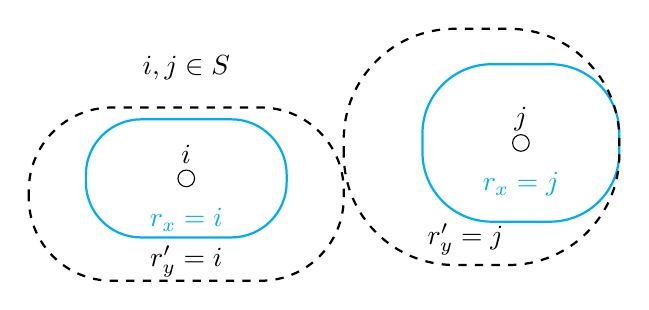
\begin{tikzpicture}

\coordinate (r1) at (2,2.4);
\coordinate (r2) at (6.25,2.85);
\coordinate (r3) at (8,2.8);

\node[] at (2, 3.8) {$i, j\in S$};
\draw (r1) circle [radius=3pt] coordinate (j);
\draw (j) node [above=.15cm] {$i$};
\draw (r2) circle [radius=3pt];
\draw (r2) node [above=.15cm] {$j$};

\node[cyan, draw, shape=rectangle, minimum width=2.55cm, minimum height=1.5cm, anchor=center,rounded corners=20pt,thick] at (r1) {};
\node[cyan] at ([yshift=-15pt]j) {$r_x = i$};
\node [cyan, draw, shape=rectangle, minimum width=2.5cm, minimum height=2.0cm, anchor=center,rounded corners=25pt,thick] at  (r2) {};
\node[cyan] at ([yshift=-15pt]r2) {$r_x = j$};

\draw[\darkorange, rounded corners=30pt,dashed,thick]
  (0,1.1) rectangle ++(4,2.2);
\node[\darkorange] at ([yshift=-30pt]j) {$r'_y = i$};
\draw[\darkorange, rounded corners=40pt,dashed,thick]
  (4,1.3) rectangle ++(3.5,3);
\node[\darkorange] at ([xshift=-20pt,yshift=-35pt]r2) {$r'_y = j$};
\end{tikzpicture}

\caption{Illustration of the data structures maintained by \growshrink.
Here we show two vertices $i, j\in S$: within the blue lines
are those vertices $x$ whose representative $r_x$ is either $i$ (on the left)
or $j$ (on the right); the vertices $y$ within the dashed orange lines, in turn,
have either $i$ or $j$ as their representative $r'_y$.}
\label{fig:grow-shrink-ds}
\end{figure}

\Cref{fig:grow-shrink-ds} illustrates an example of the data structures maintained
by the \growshrink algorithm.
Since the graph is connected, these data structures are well-defined for all
groups $S$ of size $|S| \ge 1$.
Furthermore, the sum of the differences between $d_S'(x)$ and $d_S(x)$ is exactly
the difference in farness when $r_x$ is removed from $S$. Later, we will use
this fact to quickly determine differences in farness due to the removal of
vertices from the group.

Notice that it can happen that $d_S(x) = d_S'(x)$; nevertheless, $r_x$ and
$r_x'$ are always distinct. Indeed, there can be two different vertices
$r_x,r_x' \in S$ that satisfy $d(r_x, x) = d(r_x', x) = d(S, x)$.
We also define:
%
\begin{align*}
    R_u  &:= \set{x \in V\setminus S : r_x = u},\\
    R_u' &:= \set{x \in V\setminus S : r_x' = u}.
\end{align*}

\begin{algorithm}
\caption{Overview of the \growshrink Algorithm}
\label{algo:grow-shrink}
\begin{algorithmic}[1]
\Repeat
\State approximate $D_v$ for all $v \in V \setminus S$ with Cohen's algorithm~\cite{DBLP:journals/jcss/Cohen97}
\label{line:ghc-ls-grow-1}
\State$v \gets \Sv$
\State run pruned BFS from $v$\Comment{to recompute $\gfarn(S), d,$ and $d'$}
\label{line:ghc-ls-grow-2}
\State$u \gets \argmin_{u \in S} \sum_{x \in R_u}d'(x) - d(x)$
\label{line:ghc-ls-shrink-1}
\State$S \gets \Su$
\State run Dijkstra-like algorithm\Comment{to recompute $\gfarn(S), d,$ and $d'$}
\label{line:ghc-ls-shrink-2}
\Until{previous iteration did not decrease $\gfarn(S)$}
\end{algorithmic}
\end{algorithm}



\Cref{algo:grow-shrink} gives a high-level overview of the \growshrink algorithm.
In the following, we discuss the growing phase
(\Crefrange{line:ghc-ls-grow-1}{line:ghc-ls-grow-2}) and the shrinking phase
(\Crefrange{line:ghc-ls-shrink-1}{line:ghc-ls-shrink-2}).
The time complexity of \growshrink is dominated by the Dijkstra-like algorithm in
\Cref{line:ghc-ls-shrink-2}. Therefore, it runs in $\Oh(n + m\log n)$
time per swap -- if using an appropriate priority queue.
The space complexity is $\Oh(n + m)$.

\subsection{Vertex Additions}
%
When adding a vertex $v$ to $S$, we want to select $v$ such that $\gfarn(\Sv)$
is minimized. Note that minimizing $\gfarn(\Sv)$ is equivalent to maximizing
the difference $\gfarn(S) - \gfarn(\Sv) = \deltafarnm(v)$. Instead of maximizing
$\deltafarnm(v)$, we maximize the lower bound $|D_v|\cdot d(S, v)$.
We perform a small number of iterations of Cohen's reachability set size
approximation algorithm~\cite{DBLP:journals/jcss/Cohen97}
(see \Cref{sec:lsh-gc-quality-vertex-exchanges}) to select the vertex $v$ with
(approximatively) largest $|D_v|$.

After $v$ is selected, we perform a BFS from $v$ to compute $\deltafarnm(v)$
exactly. As we only need to visit the vertices whose distance to $\Sv$ is
smaller than to $S$, the BFS can be pruned at each vertex $x$ with $d(S, x) <
d(v, x)$. During the BFS, the values $d_S, d_S', r_x,$ and $r_x'$ are updated
to reflect the vertex addition, \ie whether $v$ realizes the new distance $d_S$
or $d_S'$.

\subsection{Vertex Removals}
%
\begin{figure}
\centering
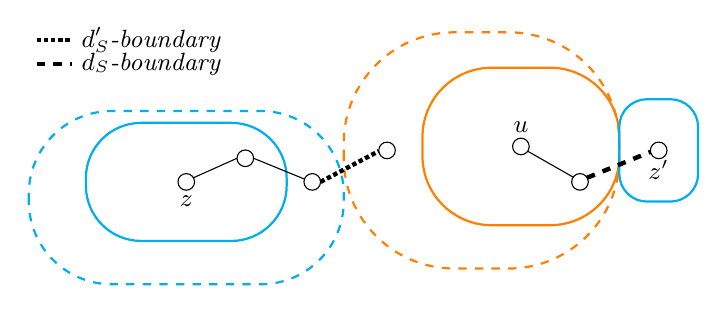
\begin{tikzpicture}
\small

\coordinate (r1) at (2,2.4);
\coordinate (r2) at (6.25,2.85);
\coordinate (r3) at (8,2.8);

\draw[cyan, rounded corners=30pt,dashed,thick]
  (0,1.1) rectangle ++(4,2.2);
\draw[orange, rounded corners=40pt,dashed,thick]
  (4,1.3) rectangle ++(3.5,3);
\node[cyan, draw, shape=rectangle, minimum width=2.55cm, minimum height=1.5cm, anchor=center,rounded corners=20pt,thick] at (r1) {};
\node [orange, draw, shape=rectangle, minimum width=2.5cm, minimum height=2.0cm, anchor=center,rounded corners=25pt,thick] at  (r2) {};
\node [cyan,draw, shape=rectangle, minimum width=1cm, minimum height=1.3cm, anchor=center,rounded corners=10pt,
thick] at (r3) {};

\draw (r1) circle [radius=3pt] coordinate (w);
\draw (w) node [below=.1cm] {$z$};
\draw (r1) ++(.75,.3) circle [radius=3pt] coordinate(w1);
\draw (w1) ++(.85,-.3) circle [radius=3pt] coordinate(w2);
\draw (w2) ++(.95,0.4) circle [radius=3pt] coordinate(w3);

\path (w) ++(30:3pt) coordinate (pw1);
\path (w1) ++(180:3pt) coordinate (pw2);
\path (w1) ++(0:3pt) coordinate (pw3);
\path (w2) ++(160:3pt) coordinate (pw4);
\path (w2) ++(0:3pt) coordinate (pw5);
\path (w3) ++(185:3pt) coordinate (pw6);

\draw[-] (pw1) -- (pw2);
\draw[-] (pw3) -- (pw4);
\draw[densely dotted, ultra thick] (pw5) -- (pw6);


\draw (r2) circle [radius=3pt];
\draw (r2) node [above=.1cm] {$u$};
\draw (r2) ++(.75,-.45) circle [radius=3pt] coordinate (u1);
\draw (r3) circle [radius=3pt];
\draw (r3) node [below=.1cm] {$z'$};

\path (r2) ++(325:3pt) coordinate (pu1);
\path (u1) ++(145:3pt) coordinate (pu2);
\path (u1) ++(30:3pt) coordinate (pu3);
\path (r3) ++(190:3pt) coordinate (pu6);

\draw[-] (pu1) -- (pu2);
\draw[dashed, ultra thick] (pu3) -- (pu6);

\coordinate (l1) at (.1, 4.2);
\coordinate (l2) at (.55, 4.2);
\coordinate (l3) at (.1, 3.9);
\coordinate (l4) at (.55, 3.9);
\draw[densely dotted, ultra thick] (l1) -- (l2);
\draw[dashed, ultra thick] (l3) -- (l4);
\draw (l2) ++(1,0) node[align=left] {$d_S'$-boundary};
\draw (l4) ++(1,0) node[align=left] {$d_S$-boundary};
\end{tikzpicture}


\caption{$z$, $u$ and $z'$ are vertices in $S$. Vertices within the solid
regions belong to $R_z$, $R_u$ and $R_{z'}$, respectively. Vertices within
the dashed regions belong to $R'_z$ and $R'_u$, respectively. After
removing $u$ from $S$, the vertices $x \in R'_u$ will have an invalid
$r_x'$ and $d_S'(x)$.}
\label{fig:lsh-gc-boundary-pair}
\end{figure}

For vertex removals, we can efficiently calculate the exact increase in farness
$\deltafarnp(u) := \gfarn(\Su) - \gfarn(S)$ for all vertices $u \in S$, even
without resorting to approximation. In fact, $\deltafarnp(u)$ is given as:
%
\[
\deltafarnp(u) = \sum_{x \in R_u}d_S'(x) - d_S(x).
\]

We need to compute $k$ such sums -- \ie $\deltafarnp(u)$ for each $u \in S$.
All of them, however, can be computed at the same time by a single linear scan
through all the vertices in $V$.

On the other hand, it is more challenging to update $d_S, d_S', r_x,$ and
$r_x'$ after the removal of a vertex $u$ from $S$. For vertices $x$ with an
invalid $d_S(x)$ -- \ie vertices $x \in R_u$ -- we can simply update $d_S(x) \gets
d_S'(x)$ and $r_x \gets r_x'$. This update invalidates $d_S'(x)$ and $r_x'$. In
the following, we treat $d_S'(x)$ as infinite and $r_x'$ as undefined for all
updated vertices $x$; eventually, those expressions will be restored to valid
values using the algorithm that we describe in the remainder of this section.
Indeed, we now have to handle all vertices with an invalid $d_S'(x)$ -- \ie
those in $R_u\cup R_u'$. This computation is more involved.
%
We run a Dijkstra-like algorithm (even in the unweighted case) to \enquote{fix}
$d_S'(x)$ and $r_S'(x)$. The following definition yields the starting point of
our Dijkstra-like algorithm.

\begin{definition}[$d_S$-boundary and $d_S'$-boundary pair]
Let $x \in V$ be any vertex and let $y \in N(x) \cap (R_u \cup R_u')$ be a neighbor
of $x$ that needs to be updated.

\begin{itemize}
    \item We call $\pair{x}{y}$ a $d_S$-boundary pair for $y$ iff $r_x \neq r_y$.
        In this case, we set $b(x, y) := d_S(x) + d(x, y)$.
    \item We call $\pair{x}{y}$ a $d_S'$-boundary pair for $y$ iff $r_x = r_y$
        and $x \notin R_u \cup R_u'$. In this case, we set $b(x, y) := d_S'(x)
        + d(x, y)$.
\end{itemize}

In both cases, we call $b(x, y)$ the \emph{boundary distance} of $\pair{x}{y}$.
\end{definition}

The definition is illustrated in \Cref{fig:lsh-gc-boundary-pair}. Intuitively,
boundary pairs define the boundary between regions of $G$ that have a valid
$d_S'(x)$ -- blue regions in \Cref{fig:lsh-gc-boundary-pair} -- and regions of the
graph that have an invalid $d_S'(y)$ -- orange region in
\Cref{fig:lsh-gc-boundary-pair}.
%
The boundary distance $b(x, y)$ corresponds to the value of $d_S'$ that a SSSP
algorithm could propagate from $x$ to $y$. We need to distinguish $d_S$-boundary
pairs and $d_S'$-boundary pairs as the boundary distance can either be
propagated on a shortest path from $S$ over $x$ to $y$ (in case of a
$d_S$-boundary pair) or on a shortest path from $S_{-r_x}$ over $x$ to $y$ (in
case of a $d_S'$-boundary pair).

Consider all $y \in V \setminus S$ such that there exists at least one
($d_S$- or $d_S'$-)boundary pair for $y$. For such $y$, let $\pair{x}{y}$ be
the boundary pair with minimal boundary distance $b(x, y)$.
Our algorithm first determines all such $y$ and updates $d_S'(y) \gets b(x,
y)$. If $\pair{x}{y}$ is a $d_S$-boundary pair, we set $r_y \gets r_x$; for
$d_S'$-boundary pairs, we set $r_y \gets r_x'$. After this initial update, we
run a Dijkstra-like algorithm starting from these vertices $y$ for which a
boundary pair exists.
%
The algorithm treats $d_S'$ as the distance. Compared to the standard Dijkstra
algorithm, ours needs the following modifications: For each vertex $x$, our
algorithm only visits those neighbors $y$ that satisfy $r_y \neq r_x'$;
furthermore, whenever such a visit results in an update of $d_S'(y)$, we
propagate $r_y' \gets r_x'$. Note that these conditions imply that we never
update $r_y'$ such that $r_y' = r_y$.

\begin{lemma}[\cite{DBLP:conf/bigdataconf/AngrimanGM19}]
\label{lemma:lsh-gc-dijkstra}
After the Dijkstra-like algorithm terminates, for all the explored vertices
$x$, $d_S'(x)$ and $r_x'$ are correct.
\end{lemma}


\section{Variants and Algorithmic Improvements}
\label{sec:lsh-gc-variants}
%
\subsection{Semi-local Swaps}
%
One weakness of the \localswaps algorithm from \Cref{sec:lsh-gc-local-swaps} is
that it only performs local vertex exchanges. Indeed, the algorithm always
swaps a vertex $u\in S$ and a vertex in $v\in N(u) \setminus S$. This condition
can be generalized: in particular, it is sufficient that $u\in S$ also satisfies
$u \in N(\Sv)$.
%
In this situation, the distances of all vertices can still only change by one
and the algorithm remains correct. Note that this naturally partitions
candidates $u$ into two sets: (i) the set $N(v) \cap S$ of candidates that
the original algorithm considers and (ii) the set $N(S) \cap S$.
Candidates in the latter set can be determined independently of $v$; indeed, they can
be swapped with any $v \in N(S) \setminus S$. Hence, our swap selection strategy
from \Cref{sec:local-swaps-choosing} continues to work with little modifications.

\subsection{Restricted Swaps}
\label{sec:lsh-gc-ls-restrict}
%
To further improve the performance of our
\localswaps algorithm at the cost of its solution quality, we consider the
following variant: instead of selecting the pair of vertices $\pair{u}{v}$ that
maximizes $|D_v| - |\Lambda_u|$, we just select the vertex $v$ that maximizes
$|D_v|$ and then choose $u \in N(v) \cap S$ such that $|\Lambda_u|$ is
minimized. This restricts, however, the choices for $u$; hence, we expect this
\emph{Restricted} \localswaps algorithm to yield solutions of worse quality.
On the other hand, due to the restriction, we also expect it to converge faster.

\subsection{\emph{Local} \growshrink}
\label{sec:lsh-gc-local-gs}
%
During exploratory experiments, it turned out that \growshrink sometimes
overestimates the lower bound $|D_v|\cdot d(S, v)$ of the decrease in
farness $\gfarn(S) - \gfarn(\Sv)$ after the addition of a vertex $v$.
%
This happens because errors in the approximation of $|D_v|$ are amplified
by the multiplication with a large $d(S, v)$. Hence, we found that restricting
the algorithm's choices for $v$ to vertices near $S$ improves the solution
quality of the algorithm.

It may seem that this variant of \growshrink makes it vulnerable to the same
weaknesses of \localswaps. Namely, local choices imply that large numbers of
exchanges might be required to reach a local optima, and it becomes hard to
escape local optima. Fortunately, additional techniques discussed in
\Cref{sec:lsh-gc-extended-gs} can be used to avoid this problem.

\subsection{\emph{Extended} \growshrink}
\label{sec:lsh-gc-extended-gs}
%
Even in the case of \growshrink, the bound of \Cref{lemma:delta-group-farness}
becomes worse for vertices at long distances from $S$. As detailed in
\Cref{sec:lsh-gc-quality-vertex-exchanges}, this happens as our reachability
set size approximation strategy does not take back edges into account.
This problem affects our algorithm especially on graphs with high diameter
where we expect that many back edges exist. We mitigate this problem -- as well
as the problems mentioned in \Cref{sec:lsh-gc-local-gs} -- by allowing the group
to grow by more than one vertex before shrink it again.
In particular, we allow the group to grow to size $k + h$ for some $h \ge 1$,
before we shrink it back to $k$.

In our experiments in \Cref{sec:lsh-gc-experiments-ls}, we consider two
strategies to choose $h$. First, we consider constant values for $h$. However,
we do not expect this to be appropriate for all graphs: specifically, we want
to take the diameter of the graph into account. Hence, a more sophisticated
strategy selects $h = \diam(G) / k^p$ for a fixed exponent $p$.
%
This strategy is inspired by mesh-like graphs (\eg real-world road networks or
other infrastructure networks): if we divide a quadratic two-dimensional mesh
$G$ into $k$ quadratic sub-meshes (where $k$ is a power of 2), the diameter of
the sub-meshes is $\diam(G) / \sqrt{k}$. Hence, if we assume that each vertex
of the group covers an equal amount of vertices in the remaining graph, $h =
\diam(G) / \sqrt{k}$ vertex additions should be sufficient to find at least
one \enquote{good} vertex that improves a size-$k$ group.
%
As we expect that large real-world networks deviate from ideal two-dimensional
meshes to some extent, we consider not only $p = 1/2$ but also other values of
$p$.


\subsection{Engineering the Reachability Set Size Approximation Algorithm}
%
Cohen's reachability set size approximation
algorithm~\cite{DBLP:journals/jcss/Cohen97} has multiple parameters that need
to be chosen appropriately. In particular, there is a choice of probability
distribution (exponential vs. uniform), the estimator function (averaging vs.
selection-based), the number of samples, and the width of each random number.
%
For the estimator, we use the averaging estimator because it can be implemented
more efficiently than a selection-based estimator -- it only requires averaging
numbers instead of finding the $k$-smallest number.
%
We performed exploratory experiments to determine a good configuration of the
remaining parameters. Our conclusions are that, while the exponential
distribution empirically offers better accuracy than the uniform distribution,
the algorithm can be implemented much more efficiently using the uniform
distribution: specifically, for the uniform distribution, it suffices to
generate and store per-vertex random numbers as (unsigned) integers, while the
exponential distribution requires floating point calculations. We compensate
the decrease in accuracy by simply gathering more samples.

For the uniform distribution in real-world graphs, 16 bits per integer turns
out to yield sufficient accuracy. In this setting, we found that 16 samples
are enough to accurately find the vertex with highest reachability set size.
%
In particular, while the theoretical guarantee in~\cite{DBLP:journals/jcss/Cohen97}
requires the number of samples to grow with $\log n$, we found this number to
have a negligible impact on the solution quality of our group-closeness
heuristic (see \Cref{sec:lsh-gc-impact-of-rss-apx}).

\subsection{Memory Latency in Reachability Set Size Approximation}
%
It is well-known that the empirical performance of graph traversal algorithms
(such as BFS and Dijkstra) is often limited by memory
latency~\cite{DBLP:conf/icpp/BaderCF05,DBLP:journals/ppl/LumsdaineGHB07}.
Unfortunately, the reachability set size approximation algorithm needs to perform
multiple traversals of the same graph. To mitigate this issue, we perform multiple
iterations of the approximation algorithm at the same time.
%
This technique reduces the running time of the algorithm at the cost of a higher
memory footprint. More precisely, during each traversal of the graph, we store 16
random integer per vertex and we aggregate all 16 minimal values per vertex at the
same time. This operation can be performed very efficiently by utilizing SIMD vector
operations. Specifically, we use 256-bit AVX operations of our Intel Xeon CPUs to
take the minimum of all 16 values at the same time. As mentioned above,
aggregating 16 random numbers per vertex is enough for our use case; thus, using SIMD
aggregation, we only need to perform a single traversal of the graph.

\subsection{Accepting Swaps and Stopping Condition}
%
As detailed in \Cref{sec:lsh-gc-local-swaps,sec:lsh-gc-grow-shrink}, our
algorithms stop once the cannot find another vertex exchange that improves the
closeness score of the current group. Exchanges that worsen the score are not
accepted. To prevent vertex exchanges that increase the group-closeness score
only negligibly, we also set a limit on the number of vertex exchanges. In our
experiments, we choose a conservative limit that does not impact the solution
quality measurably (see \Cref{sec:lsh-vertex-exc-impact}).

\section{Experimental Results}
\label{sec:lsh-gc-experiments-ls}
%
In this section, we evaluate the performance of our algorithms against the
state-of-the-art greedy algorithm by Bergamini
\etal~\cite{DBLP:conf/alenex/BergaminiGM18} -- we do not consider the naive
greedy algorithm and the OSA heuristic of~\cite{DBLP:conf/adc/ChenWW16} because
they are both dominated by~\cite{DBLP:conf/alenex/BergaminiGM18}.
We evaluate two variants, \emph{LS} and \emph{LS-restrict}
(see \Cref{sec:lsh-gc-ls-restrict}), of our \localswaps algorithm, and three variants,
\emph{GS}, \emph{GS-local} (see \Cref{sec:lsh-gc-local-gs}), and \emph{GS-extended}
(see \Cref{sec:lsh-gc-extended-gs}) of our \growshrink algorithm.
%
We evaluate these algorithms for group sizes of $k \in \set{5, 10, 20, 50, 100}$ on
the largest connected component of the input graph. We measure the performance
in terms of running time and closeness centrality of the group computed by the
algorithms.
%
Because our algorithms construct an initial group $S$ by selecting $k$ vertices
uniformly at random (see \Cref{sec:lsh-gc-preliminaries}), we average the results
of five runs, each one with a different random seed, using the geometric mean to
aggregate speedups and relative closeness scores.\footnote{These five runs are done
to average out particularly bad (or good) selections of initial groups; as one can see
from \Cref{sec:lsh-gc-impact-of-rss-apx}, the variance due to the randomized reachability set size
algorithm is negligible.}
%
Unless stated otherwise, our experiments are based on the graphs listed in
\Cref{tab:lsh-gc-heu-instances}. They are all undirected and have been downloaded
from the 9th DIMACS Challenge~\cite{demetrescu2009shortest} and
KONECT~\cite{kunegis2013konect} public repositories.
On those instances, the running time of the greedy baseline always varies
between 10 minutes to 2 hours -- detailed running times are reported in
\Cref{tab:lsh-gc-heu:times-unweighted,tab:lsh-gc-heu:times-weighted},
\Cref{sec:lsh-gc-heu:running-times}.

Our algorithms are implemented in the
NetworKit~\cite{DBLP:journals/netsci/StaudtSM16} C++ framework and use
PCG32~\cite{o2014pcg} to efficiently generate random numbers.
All experiments were executed with sequential code on a Linux machine
with an \egocpu and \egoram of memory.

\begin{table}
\centering\footnotesize
\captionabove{Networks used in the experiments.}
\label{tab:lsh-gc-heu-instances}
\begin{subtable}[t]{.6\textwidth}
\centering
\caption{Unweighted networks.}
\label{tab:lsh-gc-heu-unweighted}
\begin{tabular}{lrrr}
\toprule
Network & $n$ & $m$ & Category \\
\midrule
dimacs9-NY & \numprint{264346} & \numprint{365050} & Road\\
dimacs9-BAY & \numprint{321270} & \numprint{397415} & Road\\
web-Stanford & \numprint{255265} & \numprint{1941926} & Hyperlink\\
hyves & \numprint{1402673} & \numprint{2777419} & Social\\
youtube-links & \numprint{1134885} & \numprint{2987468} & Social\\
com-youtube & \numprint{1134890} & \numprint{2987624} & Social\\
web-Google & \numprint{855802} & \numprint{4291352} & Hyperlink\\
trec-wt10g & \numprint{1458316} & \numprint{6225033} & Hyperlink\\
dimacs10-eu-2005 & \numprint{862664} & \numprint{16138468} & Road\\
soc-pokec-relationships & \numprint{1632803} & \numprint{22301964} & Social\\
wikipedia\_link\_ca & \numprint{926588} & \numprint{27133794} & Hyperlink\\
\bottomrule
\end{tabular}

\end{subtable}\hfill
\begin{subtable}[t]{.39\textwidth}
\centering
\caption{Weighted road networks of US states.}
\label{tab:lsh-gc-heu-weighted}
\begin{tabular}{lrr}
\toprule
State & $n$ & $m$ \\
\midrule
DC & \numprint{9522} & \numprint{14807}\\
HI & \numprint{21774} & \numprint{26007}\\
AK & \numprint{48560} & \numprint{55014}\\
DE & \numprint{48812} & \numprint{59502}\\
RI & \numprint{51642} & \numprint{66650}\\
CT & \numprint{152036} & \numprint{184393}\\
ME & \numprint{187315} & \numprint{206176}\\
ND & \numprint{203583} & \numprint{249809}\\
SD & \numprint{206998} & \numprint{249828}\\
WY & \numprint{243545} & \numprint{293825}\\
ID & \numprint{265552} & \numprint{310684}\\
MD & \numprint{264378} & \numprint{312977}\\
WV & \numprint{292557} & \numprint{320708}\\
NE & \numprint{304335} & \numprint{380004}\\
\bottomrule
\end{tabular}

\end{subtable}
\end{table}

\subsection{Results for \emph{Extended} \growshrink}
\label{sec:lsh-gc-exp-extended-gs}
%
\begin{figure}[tb]
\centering
\begin{subfigure}[t]{\textwidth}
\centering
\includegraphics{./sources/plots/local-search-heu/legend-h-p-params.pdf}
\end{subfigure}

\begin{subfigure}[t]{.45\textwidth}
\centering
\includegraphics{./sources/plots/local-search-heu/speedups-h-p-params.pdf}
\caption{Speedup over the greedy algorithm (geometric mean).}
\end{subfigure}\hfill
\begin{subfigure}[t]{.45\textwidth}
\centering
\includegraphics{./sources/plots/local-search-heu/quality-h-p-params.pdf}
\caption{Closeness score relative to the score of the group returned
by greedy (geometric mean).}
\label{fig:lsh-gc-quality-h-p}
\end{subfigure}\hfill
\caption{Performance of the extended \growshrink algorithm
for different values of $h$ or $p$;
unweighted graphs, $k = 10$.}
\label{fig:lsh-gc-h-p}
\end{figure}

\begin{figure}[tb]
\centering
\begin{subfigure}[t]{.45\textwidth}
\centering
\includegraphics{./sources/plots/local-search-heu/gs-extended-time-rmat.pdf}
\caption{R-MAT networks; $2^{17}$
to $2^{24}$ vertices (up to $268$ million edges).}
\label{fig:lsh-gc-time-rmat}
\end{subfigure}\hfill
\begin{subfigure}[t]{.45\textwidth}
\centering
\includegraphics{./sources/plots/local-search-heu/gs-extended-time-rhg.pdf}
\caption{Random hyperbolic networks; $2^{17}$
to $2^{26}$ vertices (up to $671$ million edges).}
\label{fig:lsh-gc-time-rhg}
\end{subfigure}
\caption{Running time (in seconds) of the extended \growshrink algorithm on
synthetic graphs; $p = 0.75$, $k = 10$.}
\label{fig:lsh-gc-time-synthetic}
\end{figure}

In a first experiment, we evaluate the performance of our \emph{extended}
\growshrink algorithm against the greedy heuristic.
Because of its ability to escape local optima, we expect it to be the
best algorithm in terms of quality -- hence, it should be a good default
choice among our algorithms. For this experiment, we set $k = 10$.

As discussed in \Cref{sec:lsh-gc-extended-gs}, we implement two strategies
to determine $h$: we either fix a constant $h$, or we fix
a constant $p$. For both strategies, we evaluate multiple values for
$h$ or $p$; results are shown in \Cref{fig:lsh-gc-h-p}. As expected, higher
values of $h$ (or, similarly, lower values of $p$) increase the algorithm's
running time -- while $h > 1$ allows \growshrink to perform better choices,
it does not converge $h$ times as fast.
%
Still, for all tested values of $h$ or $p$, the extended \growshrink algorithm
is one to two orders of magnitude faster than the greedy baseline. Furthermore,
values of $p < 1$ yield results of very good quality: for $p = \numprint{0.75}$,
for example, we achieve a quality of $\onedigit{\gsPSevenFiveKQualNum}\%$.
%
At the same time, using this setting for $p$, our algorithm is
$\onedigit{\gsPSevenFiveKSpeed}\times$ faster than the greedy algorithm.
We remark that, for all but the smallest values of $h$ (\ie those
corresponding to the lowest quality), choosing constant $p$ is a better
strategy than choosing constant $h$: for the same running time,
constant $p$ always achieves solutions of higher quality.


\subsection{Scalability to Large Graphs}
%
\begin{table}
\captionabove{Running time of the extended \growshrink algorithm on
large real-world networks; $p = \numprint{0.75}$, $k = 10$.}
\label{tab:lsh-gc-heu-time-large}
\centering\smallskip\footnotesize

\begin{tabular}{lrrr}
\toprule
Network & $n$ & $m$ & Time (s) \\
\midrule
soc-LiveJournal1 & \numprint{4843953} & \numprint{42845684} & \numprint{95.3}\\
livejournal-links & \numprint{5189808} & \numprint{48687945} & \numprint{135.6}\\
orkut-links & \numprint{3072441} & \numprint{117184899} & \numprint{199.9}\\
dbpedia-link & \numprint{18265512} & \numprint{126888089} & \numprint{368.0}\\
dimacs10-uk-2002 & \numprint{18459128} & \numprint{261556721} & \numprint{333.1}\\
wikipedia\_link\_en & \numprint{13591759} & \numprint{334640259} & \numprint{680.1}\\
\bottomrule
\end{tabular}

\end{table}

We also analyze the running time of our extended \growshrink algorithm
on large-scale networks. To this end, we switch to graphs larger than
the ones in \Cref{tab:lsh-gc-heu-instances}. We fix $p = \numprint{0.75}$,
as \Cref{sec:lsh-gc-exp-extended-gs} demonstrated that this setting results
in a favorable trade-off between solution quality and running time.
%
The greedy algorithm is not included in this experiments as it requires
multiple hours of running time, even for the smallest real-world graphs
we consider in these experiments.

\paragraph{Results on Synthetic Data}
%
\Cref{fig:lsh-gc-time-synthetic} shows the average running time of our algorithm
on randomly generated R-MAT~\cite{DBLP:conf/sdm/ChakrabartiZF04} as well as
graphs from a generator for random hyperbolic
graphs~\cite{DBLP:conf/hpec/LoozOLM16}.\footnote{Like R-MAT, the random
hyperbolic model yields graphs with a skewed degree distribution, similar to
the one found in real-world complex networks.} For the R-MAT generator, we use
the same parameter setting as in
the Graph 500's benchmark~\cite{murphy2010introducing}
-- \ie \graphfh. Concerning the random hyperbolic
generator, we set the average degree to 20, and the exponent of the power-law
degree distribution to 3.

In the (log-log) plot, the straight lines represent a linear
regression of the running times. In both cases, the running time curves are
almost as steep as the regression line, \ie the running time grows linearly in
the number of vertices for the considered network models and sizes.

\paragraph{Results on Large Real-World Datasets}
%
\Cref{tab:lsh-gc-heu-time-large} reports the algorithm's performance
on large real-world graphs. In contrast to the greedy algorithm -- which
would requires hours, our extended \growshrink algorithm handles real-world
networks with hundreds of millions of edges in a few minutes. For the
\emph{orkut-links} network, Bergamini \etal~\cite{DBLP:conf/alenex/BergaminiGM18}
report running times for the greedy of \emph{16 hours} on their machine --
it is the largest instance in their experiments.

\subsection{Accelerating Performance on Unweighted Graphs}
%
\begin{figure}[tb]
\centering
\begin{subfigure}[t]{\textwidth}
\centering
\includegraphics{./sources/plots/local-search-heu/legend-unweighted.pdf}
\end{subfigure}
\centering
\begin{subfigure}[t]{.45\textwidth}
\centering
\includegraphics{./sources/plots/local-search-heu/speedups-unweighted.pdf}
\caption{Speedup over the greedy algorithm (geometric mean).}
\label{fig:lsh-gc-speedup-unweighted}
\end{subfigure}\hfill
\begin{subfigure}[t]{.5\textwidth}
\centering
\includegraphics{./sources/plots/local-search-heu/quality-unweighted.pdf}
\caption{Closeness score relative to the score of the group returned by greedy
(geometric mean).}
\label{fig:lsh-gc-quality-unweighted}
\end{subfigure}
\caption{Performance of our local search algorithms for different values of $k$;
unweighted graphs.}
\label{fig:lsh-gc-perf-unweighted}
\end{figure}

While the extended \growshrink algorithm yields results with very high quality,
if quality is not a primary concern, even faster algorithms might be desirable
for very large graphs. To this end, we also evaluate the performance of the
non-extended \growshrink and the \localswaps algorithms.
%
For extended \growshrink, we fix $p = \numprint{0.75}$ again.
The speedup and the quality of our algorithms over the greedy baseline, for different
values of the group size $k$, are shown in
\Cref{fig:lsh-gc-speedup-unweighted,fig:lsh-gc-quality-unweighted}, respectively.
Note that the greedy algorithm scales well for large $k$, so that the speedup of
our algorithms decreases with $k$.\footnote{Indeed, as mentioned in \Cref{sec:lsh-gc-intro},
the main bottleneck of the greedy algorithm is adding the first vertex into the group.}
However, even for large groups of $k = 100$, all of our algorithms are still at
least $\onedigit{\minSpeedupKHundred}\times$ faster.

Our non-extended local version of \growshrink is the next best algorithm after
extended \growshrink. As explained in \Cref{sec:lsh-gc-local-gs}, this variant
gives better solutions than non-local \growshrink; further, it achieves a
speedup of $\onedigit{\gsLocalSpeedupOverNonLocal}\times$ over extended
\growshrink with $p = 0.75$ and $k = 10$ -- and a speedup of
$\onedigit{\gsLocalSpeedKTen}\times$ over greedy. The solution quality in this case
is $\onedigit{\gsLocalQualKTen}\%$ of the greedy quality.

The non-restricted \localswaps algorithm is dominated by \growshrink,
both in terms of running time and solution quality. Furthermore, compared
to other algorithms, the restricted \localswaps algorithm only gives a rough
estimate of the group with highest closeness; it is, however, significantly faster
than all other algorithms and may be employed in exploratory analysis of
graph datasets.

\subsection{Results on Weighted Road Networks}
%
\begin{figure}[tb]
\centering
\begin{subfigure}[t]{\textwidth}
\centering
\includegraphics{./sources/plots/local-search-heu/legend-weighted.pdf}
\end{subfigure}
\centering
\begin{subfigure}[t]{.4\textwidth}
\centering
\includegraphics{./sources/plots/local-search-heu/speedups-weighted.pdf}
\caption{Speedup over the greedy algorithm (geometric mean).}
\label{fig:lsh-gc-speedup-weighted}
\end{subfigure}%
\hfill
\begin{subfigure}[t]{.4\textwidth}
\centering
\includegraphics{./sources/plots/local-search-heu/quality-weighted.pdf}
\caption{Closeness score relative to the score of the group returned by greedy (geometric mean).}
\label{fig:lsh-gc-quality-weighted}
\end{subfigure}
\caption{Performance of our local search algorithms for different values of $k$;
weighted graphs.}
\label{fig:lsh-gc-perf-weighted}
\end{figure}

Recall that the \localswaps algorithm does not support weighted graphs; thus,
in the weighted case, we report only \growshrink data.
The performance of \growshrink and local \growshrink on weighted graphs is
shown in \Cref{fig:lsh-gc-perf-weighted}. In contrast to the unweighted case,
the quality of the non-local \growshrink algorithm is superior to the greedy
baseline for all the considered group sizes. Furthermore, contrary to
unweighted graphs, the ability to perform non-local vertex exchanges greatly
benefits the non-local \growshrink compared to local \growshrink.\footnote{For
this reason, we do not include the extended \growshrink in this experiment.
In fact, we expect that it improves only slightly on GS-local (red line/bars
in \Cref{fig:lsh-gc-perf-weighted}) but cannot compete with (non-local) GS:
indeed, the ability of performing non-local vertex exchanges, as done by
GS (green line/bars in \Cref{fig:lsh-gc-perf-weighted}) appears to be
crucial to obtain high-quality results on weighted graphs.}
%
Thus, on the weighed graphs in our benchmark set, \growshrink clearly dominates
both the greedy and the local \growshrink algorithms -- both in terms of speedup
\emph{and} solution quality.


\section{Additional Experiments}
\subsection{Impact of the number of vertex exchanges}
\label{sec:lsh-vertex-exc-impact}
%
\begin{figure}[tb]
\centering
\begin{subfigure}[t]{\textwidth}
\centering
\includegraphics{./sources/plots/local-search-heu/legend-unweighted.pdf}
\end{subfigure}
\centering
\begin{subfigure}[t]{.5\textwidth}
\centering
\includegraphics{./sources/plots/local-search-heu/impact-num-exchanges-unweighted.pdf}
\caption{Unweighted graphs.}
\label{fig:lsh-gc-num-exchanges-unweighted}
\end{subfigure}\hfill
\begin{subfigure}[t]{.5\textwidth}
\centering
\includegraphics{./sources/plots/local-search-heu/impact-num-exchanges-weighted.pdf}
\caption{Weighted graphs.}
\label{fig:lsh-gc-num-exchanges-weighted}
\end{subfigure}
\caption{Behavior of the relative closeness score
(compared to the group returned by greedy, geometric mean)
over the execution of the algorithms (in terms of vertex exchanges); $k = 10$.}
\label{fig:lsh-gc-num-exchanges}
\end{figure}

\Cref{fig:lsh-gc-num-exchanges-unweighted,fig:lsh-gc-num-exchanges-weighted} depict
the closeness score relative to the one of the group computed by the greedy algorithm
depending on number of vertex exchanges performed by the algorithm. Again, for extended
\growshrink, we fix $p = \numprint{0.75}$. All of the local search algorithms quickly
converge to a value near their final result -- additional exchanges improve the
closeness score by small amounts. Thus, in order to avoid an excessive number of iterations,
setting a limit on the number on the number of vertex exchanges seems a reasonable choice.
In our experiments, we set a conservative limit of 100 exchanges.

\subsection{Impact of reachability set size approximation}
\label{sec:lsh-gc-impact-of-rss-apx}
%
\begin{figure}
\centering
\begin{subfigure}[t]{\columnwidth}
\centering
\includegraphics{./sources/plots/local-search-heu/legend-weighted.pdf}
\end{subfigure}

\begin{subfigure}[t]{.45\columnwidth}
\centering
\includegraphics{./sources/plots/local-search-heu/reach-set-size-apx-speedups.pdf}
\caption{Speedup over the greedy algorithm (geometric mean).}
\label{fig:lsh-gc-reach-set-size-apx-speedup}
\end{subfigure}\hfill
\begin{subfigure}[t]{.45\columnwidth}
\centering
\includegraphics{./sources/plots/local-search-heu/reach-set-size-apx-quality.pdf}
\caption{Closeness score relative to the score of the group returned by greedy (geom. mean).}
\label{fig:lsh-gc-reach-set-size-apx-quality}
\end{subfigure}
\caption{Performance of the \growshrink
algorithm for different numbers of samples to estimate
reachability set size; $k = 10$.}
\label{fig:lsh-gc-reach-set-size-apx}
\end{figure}

As mentioned in \Cref{sec:lsh-gc-local-gs}, the errors in the approximation of $|D_v|$ are
amplified by the multiplication with $d(S, v)$. This results in GS-local computing
higher quality solutions than GS. We study how increasing the accuracy of the reachability
set size approximation by increasing the number of samples impacts the performances
of both GS and GS-local.
\Cref{fig:lsh-gc-reach-set-size-apx-speedup} shows that GS needs at least 64 samples to
converge to a better local optimum than GS-local. However, in both cases increasing the
number of samples degrades the speedup without leading to a substantial quality
improvement (see \Cref{fig:lsh-gc-reach-set-size-apx-quality}).

\subsection{Summary of Experimental Results}
%
On unweighted graphs, a good trade-off between running time and solution quality is achieved
by the extended \growshrink algorithm with constant $p = \numprint{0.75}$.
This strategy yields solutions with at least $\onedigit{\gsPSevenFiveKQualNum}\%$
of the closeness score of a greedy solution -- greedy, in turn, was at most $3\%$ away from
the optimum on small networks in previous work~\cite{DBLP:conf/alenex/BergaminiGM18}.
%
With $k = 10$, extended \growshrink is $\onedigit{\gsPSevenFiveKSpeed}\times$
faster than greedy. Thus, it is able to handle graphs with hundreds of millions of edges
in a few minutes -- while the state of the art needs multiple hours.
%
Further, if a fast but inaccurate algorithm is needed for applications such as exploratory
analysis of graph datasets, we recommend to use the non-extended \growshrink algorithm, or,
if only a very coarse estimate of the group with maximal closeness is needed, restricted
\localswaps.

On weighted graphs, our recommendation is always to use our \growshrink algorithm, as it
outperforms the greedy state of the art both in terms of quality -- yielding solutions
that are on average $\onedigit{\wGSQualInc}\%$ better than greedy solutions --
and in terms of running time performance -- with a speedup of two orders of magnitude,
at the same time.

\section{Conclusions}
%
In this chapter, we introduced two new families of
local search algorithms for group-closeness maximization in large networks.
As maximizing group-closeness exactly is infeasible for graphs with more than
a few thousand edges, our algorithms are heuristics -- just like the state-of-the-art
greedy algorithm~\cite{DBLP:conf/alenex/BergaminiGM18}. However, for small
real-world networks where the optimum can be computed reasonably fast, the
results are empirically known to be close to optimal
solutions~\cite{DBLP:conf/alenex/BergaminiGM18}.

Compared to previous state-of-the-art heuristics, our algorithm (extended
\growshrink in particular) allow\change{s} to find groups with high closeness centrality
in real-world networks with hundreds of millions of edges in seconds to minutes
instead of multiple hours, while sacrificing less than $1\%$ in quality. In
weighted graphs, \growshrink (GS) even dominates the best known heuristic: the
GS solution quality is more than $10\%$ higher and GS is two orders of
magnitude faster.
